\subsection{自然同型}
  次に自然変換や関手を用いた量化された同型である自然同型を見ていく。
  \begin{define}[自然同型(関手の同型)]
    関手圏$\funccat{C}{D}$の対象$F,G$の同型$F\cong G$を\textbf{自然同型}と呼ぶ。また同型射となる自然変換を\textbf{同型自然変換}と呼ぶことにする。
  \end{define}
  \begin{prop}[自然同型と対象の同型]
    関手$\functor{F,G}{C}{D}$が自然同型$\iff$圏$\cat{C}$の任意の対象$A$において、ある同型射$\mor{i_A}{FA}{GA}$が存在し、$\cat{C}$の任意の射$\mor{f}{A}{B}$に対して\[i_B\circ Ff=Gf\circ i_A\]が成り立つ。
  \end{prop}
  自明に思えるが念の為証明しておく。
  \begin{proof}[$\Longrightarrow$]
    同型の定義により、ある自然変換$\nat{i}{F}{G}$、$\nat{i^{-1}}{G}{F}$が存在し、\[i\cdot i^{-1}=ID_G,\ i^{-1}\cdot i=ID_F\]が成り立つ。
    この二つの自然変換の等式を成分に分解すると、任意の対象$A$に対して\[i_A\circ i^{-1}_A=id_{GA},\ i^{-1}_A\circ i_A=id_{FA}\]が成り立つ。よって任意の対象$A$に対して同型射$i_A$が存在することが分かった。
    また$i_B\circ Ff=Gf\circ i_A$は自然変換$i$の自然性より明らかに成り立つ。
  \end{proof}
  \begin{proof}[$\Longleftarrow$]
    圏$\cat{C}$の任意の対象$A$に対して射$\mor{i_A}{FA}{GA}$が存在し、自然性として$i_B\circ Ff=Gf\circ i_A$を満たすから$i$は自然変換$\nat{i}{F}{G}$である。また同型射の逆射$i^{-1}_A$も存在する。
    自然性については、等式の両辺にそれぞれ逆射を合成して、
    \begin{align*}
      i_B\circ Ff &=Gf\circ i_A\\
      i^{-1}_B\circ (i_B\circ Ff)\circ i_A &=i^{-1}_B\circ(Gf\circ i_A)\circ i_A&\text{(射の合成の写像性)}\\
      (i^{-1}_B\circ i_B)\circ Ff\circ i_A &=i^{-1}_B\circ Gf\circ (i_A\circ i_A)&\text{(結合則)}\\
      Ff\circ i_A&=i^{-1}_B\circ Gf&\text{(同型射の定義)}
    \end{align*}
    となり、逆射も自然性を持ち、自然変換とみなせる。
    また、任意の対象$A$に対して\[i_A\circ i^{-1}_A=id_{GA},\ i^{-1}_A\circ i_A=id_{FA}\]が成り立つから、\[i\cdot i^{-1}=ID_G,\ i^{-1}\cdot i=ID_F\]が成り立ち、$F,G$は自然同型となる。
  \end{proof}
  自然同型を後者で捉える場合、$FA\cong GA$が$A$に対して自然であると述べることがある。

  複数の対象において成り立つような同型を一組の自然変換の同型で表現することができるため、これは同型という性質の量化と言える。
  対象の同型を考えるだけならば自然性を仮定する必要は無いが、自然性を満たすのであれば射集合も同型となり、$Ff\sim Gf$が成り立つ。そして実はこの対応もまた自然同型になる。
  \begin{prop}[自然同型と射集合の対応]
    関手$\functor{F,G}{C}{D}$に対して、
    $F\cong G\Longrightarrow\arset{C}{F-}{F-}\cong\arset{C}{G-}{G-}$\\
    言い換えると、圏$\cat{D}$において$FA\cong GA$が任意の$A$に対して自然である時、$\cat{Set}$において$\arset{D}{FA}{FB}\cong\arset{D}{GA}{GB}$
  \end{prop}
  \begin{proof}
    $F,G$の同型射となる自然変換をそれぞれ$\nat{i}{F}{G},\ \nat{i^{-1}}{G}{F}$とする。
    射集合の同型射をそれぞれ\[\mor{\arset{D}{i^{-1}_A}{i_B}}{\arset{D}{FA}{FB}}{\arset{D}{GA}{GB}},\ \mor{\arset{D}{i_A}{i^{-1}_B}}{\arset{D}{GA}{GB}}{\arset{D}{FA}{FB}}\]とすると、双射写像の合成より\[\arset{D}{i^{-1}_A}{i_B}\circ\arset{D}{i_A}{i^{-1}_B}=\arset{D}{i_A\circ i^{-1}_A}{i_B\circ i^{-1}_B}=\arset{D}{id_{GA}}{id_{GB}}=id_{\arset{D}{GA}{GB}}\]となる。同様に$\arset{D}{i_A}{i^{-1}_B}\circ\arset{D}{i^{-1}_A}{i_B}=id_{\arset{D}{FA}{FB}}$も示せるから、任意の対象$A,B$において$\arset{D}{FA}{FB}\cong\arset{D}{GA}{GB}$である。
    \begin{center}
      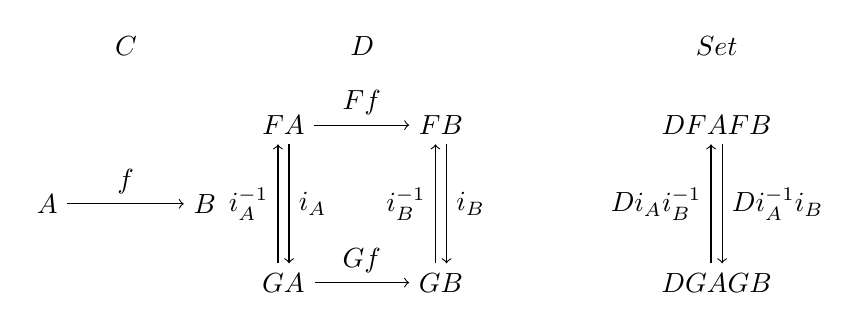
\begin{tikzpicture}[auto]
        \node (catc) at (0, 1) {$\cat{C}$};
        \node (A) at (-1, -1) {$A$};
        \node (B) at (1, -1) {$B$};
        \node (catd) at (3, 1) {$\cat{D}$};
        \node (FA) at (2, 0) {$FA$};
        \node (FB) at (4, 0) {$FB$};
        \node (GA) at (2, -2) {$GA$};
        \node (GB) at (4, -2) {$GB$};
        \node (catset) at (7.5, 1) {$\cat{Set}$};

        \node (FAFB) at (7.5, 0) {$\arset{D}{FA}{FB}$};
        \node (GAGB) at (7.5, -2) {$\arset{D}{GA}{GB}$};

        \draw[->] (A) to node{$f$}(B);
        \draw[->] (FA) to node{$Ff$}(FB);
        \draw[->] (GA) to node{$Gf$}(GB);
        \draw[->,transform canvas={xshift=2pt}] (FA) to node{$i_A$}(GA);
        \draw[->,transform canvas={xshift=2pt}] (FB) to node{$i_B$}(GB);
        \draw[->,transform canvas={xshift=-2pt}] (GA) to node{$i^{-1}_A$}(FA);
        \draw[->,transform canvas={xshift=-2pt}] (GB) to node{$i^{-1}_B$}(FB);
        \draw[->,transform canvas={xshift=2pt}] (FAFB) to node{$\arset{D}{i^{-1}_A}{i_B}$}(GAGB);
        \draw[->,transform canvas={xshift=-2pt}] (GAGB) to node{$\arset{D}{i_A}{i^{-1}_B}$}(FAFB);
      \end{tikzpicture}
    \end{center}
    次に$\arset{D}{FA}{FB}\cong\arset{D}{GA}{GB}$の$A,B$に対する自然性を証明する。\\
    すなわち、以下の図式が任意の射$\mor{g}{A'}{A},\ \mor{h}{B}{B'}$において可換になれば良い。
    \begin{center}
      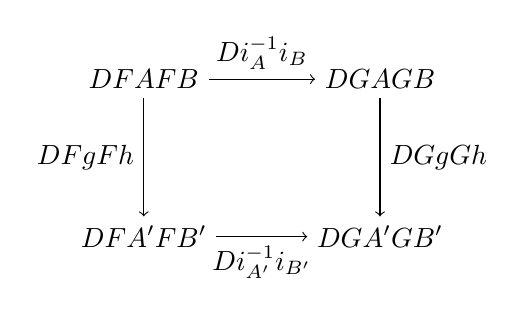
\begin{tikzpicture}[auto]
        \node (fab) at (0, 0) {$\arset{D}{FA}{FB}$};
        \node (gab) at (3, 0) {$\arset{D}{GA}{GB}$};
        \node (fab') at (0, -2) {$\arset{D}{FA'}{FB'}$};
        \node (gab') at (3, -2) {$\arset{D}{GA'}{GB'}$};

        \draw[->] (fab) to node{$\arset{D}{i^{-1}_A}{i_B}$}(gab);
        \draw[->] (fab') to node[swap]{$\arset{D}{i^{-1}_{A'}}{i_{B'}}$}(gab');
        \draw[->] (fab) to node[swap]{$\arset{D}{Fg}{Fh}$}(fab');
        \draw[->] (gab) to node{$\arset{D}{Gg}{Gh}$}(gab');
      \end{tikzpicture}
    \end{center}
    自然性の等式としては\[\arset{D}{Gg}{Gh}\circ\arset{D}{i^{-1}_A}{i_B} = \arset{D}{i^{-1}_{A'}}{i_{B'}}\circ \arset{D}{Fg}{Fh}\]のように書くことができ、射写像を合成して
    \[\arset{D}{i^{-1}_A\circ Gg}{Gh\circ i_B}=\arset{D}{Fg\circ i_{A'}^{-1}}{i_{B'}\circ Fh}\]が得られる。つまり二等式
    \[i^{-1}_A\circ Gg=Fg\circ i_{A'}^{-1},\ Gh\circ i_B=i_{B'}\circ Fh\]を示せばよい。しかしこれは自然変換$\nat{i}{F}{G},\ \nat{i^{-1}}{G}{F}$の自然性そのものであり成り立つ。よってが$\arset{D}{FA}{FB}\cong\arset{D}{GA}{GB}$の$A,B$に対して自然であることを示せた。
  \end{proof}
  心当たりがあるかもしれないが、今まで扱ってきた複数の対象において成り立つような同型のほとんどが自然同型である。次はこれらを例として確かめていく。
  \begin{prop}[$A\times 1\cong A$の自然性]
    $A\times 1\cong A$は$A$において自然である。
  \end{prop}
  \begin{proof}
    $A\times 1\cong A$の同型射はそれぞれ$\mor{\pi_{L,A\times 1}}{A\times 1}{A}$、$\mor{\tuple{id_A,!_A}}{A}{A\times 1}$であった。自然変換の始域と終域はそれぞれ恒等関手と積関手で表せそうである。

    実際に関手$\functor{Id_\cat{C}}{C}{C}$と$\functor{(-)\times 1}{C}{C}$の間の自然変換$\nat{\pi_L}{(-)\times 1}{Id_\cat{C}}$は任意の対象$A$に対して$(\pi_L)_A=\pi_{L,A\times 1}=\pi_A$と定義できる。自然同型の定義より、自然性を示すのは片方の自然変換だけで良いから、この$\pi_L$が自然性を満たすことを確かめる。
    \begin{align*}
      (\pi_L)_{B}\circ ((-)\times 1)(f)&=\pi_B\circ(f\times id_1)&\text{(自然変換と関手の定義)}\\
      &=\pi_B\circ\tuple{f\circ\pi_A,id_1\circ\pi_1}&\text{(射の積の定義)}\\
      &=f\circ\pi_A&\text{(積の普遍性)}\\
      &=Id(f)\circ(\pi_L)_A&\text{(自然変換と関手の定義)}
    \end{align*}
    よって$\pi_L$は自然変換であり、$A\times 1\cong A$は自然同型である。
    \begin{center}
      \begin{tikzpicture}[auto]
        \node (A) at (0, 0.75) {$A$};
        \node (B) at (1.5, 0.75) {$B$};
        \node (FA) at (3, 1.5) {$A\times 1$};
        \node (FB) at (4.5, 1.5) {$B\times 1$};
        \node (GA) at (3, 0) {$A$};
        \node (GB) at (4.5, 0) {$B$};

        \node (catc) at (0.75, 3) {$\cat{C}$};
        \node (catd) at (3.75, 3) {$\cat{C}$};

        \draw[->] (A) to node{$f$}(B);
        \draw[->] (FA) to node{$f\times id_1$}(FB);
        \draw[->] (GA) to node{$f$}(GB);
        \draw[->] (FA) to node{$\pi_A$}(GA);
        \draw[->] (FB) to node{$\pi_B$}(GB);

        \draw[->,bend left = 30] (catc) to node (funcf){$(-)\times 1$}(catd);
        \draw[->,bend right = 30] (catc) to node (funcg)[swap]{$Id_\cat{C}$}(catd);
        \draw[double,double equal sign distance,-implies,shorten >=5pt,shorten <=5pt] (funcf) -- node[label=right:$\pi_L$] {} (funcg);
      \end{tikzpicture}
    \end{center}

  \end{proof}
  \begin{prop}[$\arset{C}{X}{B}\cong\arset{C}{X}{B'}$の自然性]
    $B\cong B'\Longrightarrow \arset{C}{X}{B}\cong\arset{C}{X}{B'}$かつ$X$に対して自然。
  \end{prop}
  \begin{proof}[$\Longrightarrow$]
    $B\cong B'\Longrightarrow \arset{C}{X}{B}\cong\arset{C}{X}{B'}$はすでに示してあるので、同型射$\mor{\arset{C}{X}{i}}{\arset{C}{X}{B}}{\arset{Set}{X}{B'}}$が$X$に対して自然であることを示せば良い。\\
    任意の射$\mor{g}{Y}{X}$に対して、$\arset{C}{g}{B'}\circ\arset{C}{X}{i}=\arset{C}{Y}{i}\circ\arset{C}{g}{B}$が成り立つことを示せばよいが、双Hom関手の定義より\[\arset{C}{g}{i}=\arset{C}{g}{B'}\circ\arset{C}{X}{i}=\arset{C}{Y}{i}\circ\arset{C}{g}{B}\]が成り立つから明らかに自然である。
    \begin{center}
      \begin{tikzpicture}[auto]
        \node (A) at (-4, 5) {$X$};
        \node (B) at (-2, 5) {$Y$};
        \node (FA') at (0, 6) {$\arset{C}{X}{B}$};
        \node (FB') at (0, 4) {$\arset{C}{X}{B'}$};
        \node (GA') at (2, 6) {$\arset{C}{Y}{B}$};
        \node (GB') at (2, 4) {$\arset{C}{Y}{B'}$};

        \node (catc) at (-3, 8) {$\cat{C}$};
        \node (catd) at (1, 8) {$\cat{D}$};
  
        \draw[->] (A) to node{$i$}(B);

        \draw[->] (FA') to node{$\arset{C}{X}{i}$}(FB');
        \draw[->] (GA') to node{$\arset{C}{Y}{i}$}(GB');
        \draw[->] (FA') to node[swap]{$\arset{C}{g}{B}$}(GA');
        \draw[->] (FB') to node{$\arset{C}{g}{B'}$}(GB');
        \draw[->,bend left = 20] (catc) to node (funcf){$\arset{C}{-}{B}$}(catd);
        \draw[->,bend right = 20] (catc) to node (funcg)[swap]{$\arset{C}{-}{B'}$}(catd);
        \draw[double,double equal sign distance,-implies,shorten >=5pt,shorten <=5pt] (funcf) -- node[label=right:$\arset{C}{-}{i}$] {} (funcg);
      \end{tikzpicture}
    \end{center}
    この自然性が述べていることは、$\mor{f}{X}{B}$と対応する射$\mor{f'}{X}{B'}$、すなわち$f'=i\circ f,\ f=i^{-1}\circ f'$となる二射に対して、ある射$\mor{g}{Y}{X}$を両方に合成しても$f\circ g$と$f'\circ g$がまた対応することを示している。実際に計算すれば自明なことではあるが、射の前からの合成は射$f,f'$の対応関係を保つということが言える。
  \end{proof}
  \begin{proof}[$\Longleftarrow$]
    現在自然変換$\nat{\alpha}{\arset{C}{-}{B}}{\arset{C}{-}{B'}}$とその逆射$\nat{\alpha^{-1}}{\arset{C}{-}{B'}}{\arset{C}{-}{B}}$が与えられている。\\
    この二つの自然変換から$B$と$B'$の間の同型射を構成しなければ行けないが、$\alpha,\alpha^{-1}$の成分は射写像とは限らない。そのため少し工夫が必要になる。\\
    証明の方向性を示す。上の証明によると、$\mor{\arset{C}{X}{i}}{\arset{C}{X}{B}}{\arset{C}{X}{B'}}$が自然変換の$X$成分だった。この射から元の同型射である$i$を導出したい。ここでこの自然変換の$B$成分$\mor{\arset{C}{B}{i}}{\arset{C}{B}{B}}{\arset{C}{B}{B'}}$に恒等射$\mor{id_B}{B}{B}$を適用すると、射写像の定義より、$\arset{C}{B}{i}(id_B)=i$が成り立つ。\\
    これによって自然変換$\alpha,\alpha^{-1}$から元の同型射を取り出せば良い。\\
    $i=\alpha_B(id_B),\ i^{-1}=\alpha_{B'}^{-1}(id_B)$とし、$i,i^{-1}$が同型射になることを示す。$\alpha,\alpha^{-1}$の自然性より、\[\arset{C}{i^{-1}}{B'}\circ\alpha_B=\alpha_{B'}\circ\arset{C}{i^{-1}}{B}\]が成り立つ。両辺に恒等射$id_B$を適用して、
    \begin{align*}
      (\arset{C}{i^{-1}}{B'}\circ\alpha_B)id_B&=\arset{C}{i^{-1}}{B'}(i)&\text{($i$の定義)}\\
      &=i\circ i^{-1}&\text{(射写像の定義)}\\
      (\alpha_{B'}\circ\arset{C}{i^{-1}}{B})id_B&=\alpha_{B'}(i^{-1})&\text{(射写像の定義)}\\
      &=\alpha_{B'}(\alpha_{B'}^{-1}(id_B))&\text{($i^{-1}$の定義)}\\
      &=(\alpha_{B'}\circ\alpha_{B})(id_B)&\text{(写像の合成の定義)}\\
      &=id_{B'}
    \end{align*}
    よって$i\circ i^{-1}=id_{B'}$が示せた。同様に$i^{-1}\circ i=id_B$も成り立つため、$B\cong B'$が示せた。
  \end{proof}
  この証明のように、射集合が関わる自然変換の議論において恒等射が取れるように成分を指定する、というテクニックはよく使われている。この証明の核である$\arset{C}{B}{i}(id_B)=i$のより形式的な証明は、以前示した余評価射による恒等射の定義が用いられるので、興味があれば豊穣圏における弱米田の補題の証明あたりを読んでほしい。
  \begin{prop}[$\arset{C}{X}{A\times B}\cong \arset{C}{X}{A}\times \arset{C}{X}{B}$の自然性] \\
    $A\times B$が$A,B$における積対象$\iff\arset{C}{X}{A\times B}\cong \arset{C}{X}{A}\times \arset{C}{X}{B}$が$X$に対して自然
  \end{prop}
  \begin{prop}[$\arset{C}{X}{1}\cong I$の自然性] \\
    $1$が終対象$\iff\arset{C}{X}{1}\cong I$が$X$に対して自然
  \end{prop}